%!TEX root = ../main.tex

\begin{frame}{Resultados Parciais}
 \begin{itemize}
   \item Utilização de um servidor para treinamento das CNNs:
    \begin{itemize}
      \item Processador Intel Core i7
      \item 16 GB de RAM
      \item GPU Nvidia GeForce GTX 1080 com 11 GB de memória
    \end{itemize}
    \bigskip
    \item \alert{LeNet} e \alert{AlexNet}
    \bigskip
    \item Modelos degenerados tiveram seus resultados descartados
    \begin{itemize}
      \item \emph{Dying ReLU problem}
      \item Permanência em mínimos locais no treinamento
    \end{itemize}
   \end{itemize}
\end{frame}

\begin{frame}{LeNet}

  \begin{table}
  \centering
  \caption{Detalhamento dos melhores modelos obtidos com a arquitetura LeNet.}
  \label{tab:lenet}
  \begin{tabular}{cccccc}
  \toprule
  \textbf{Identificação} & \textbf{Otimizador} & \textbf{\emph{Patience}}  & \textbf{Função de Ativação} & \textbf{Acurácia} & \textbf{F-Score} \\
  \midrule
  LeNet A & RMSprop & 5 & \emph{Leaky} ReLU & $0.9865$ & $0.9755$ \\
  LeNet B & RMSprop & 15 & ReLU & $0.9858$ & $0.9740$\\
  LeNet C & SGD & 5 & ELU & $0.9787$ & $0.9619$ \\
  LeNet D & RMSprop & 10 & SELU & $0.9707$ & $0.9483$ \\
  \bottomrule
  \end{tabular}
  \end{table}

\end{frame}

\begin{frame}{LeNet}

  \begin{figure}[ht!]
      \caption{Histórico de \emph{loss} e acurácia durante o treinamento dos melhores modelos obtidos com a arquitetura LeNet.}\label{fig:lenet-treinamento}
      \begin{subfigure}[hb]{0.4\linewidth}
        \caption{\emph{Loss} durante o treinamento da LeNet A}
        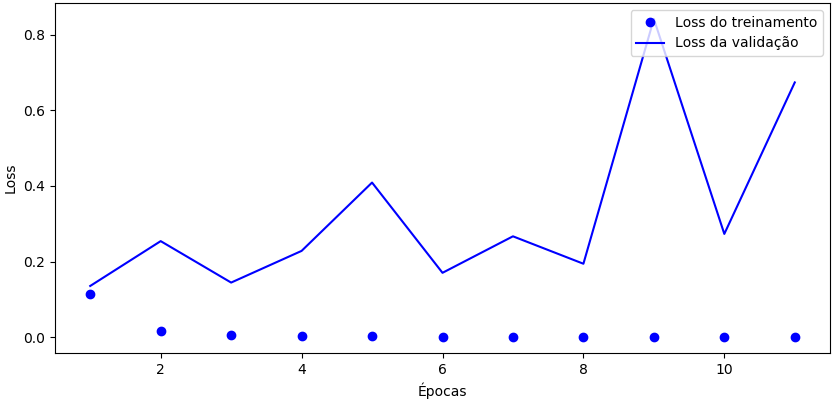
\includegraphics[width=\linewidth]{img/lenet-a-loss}
      \end{subfigure}
      \hspace{2cm}
      \begin{subfigure}[hb]{0.4\linewidth}
        \caption{Acurácia durante o treinamento da LeNet A}
        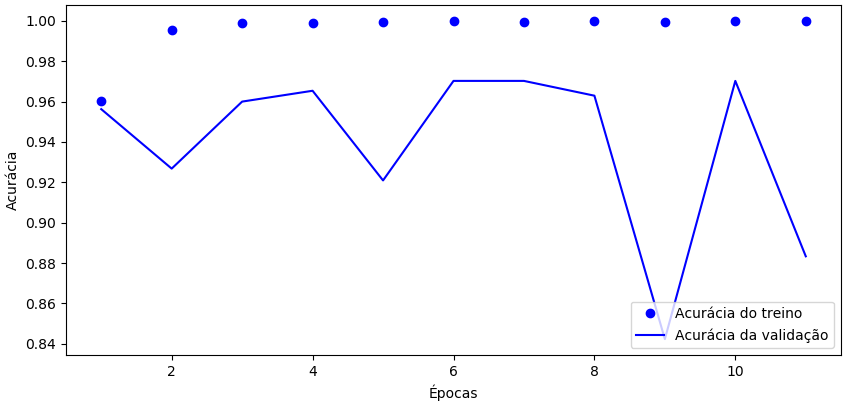
\includegraphics[width=\linewidth]{img/lenet-a-acc}%
      \end{subfigure}
  \end{figure}
\end{frame}

\begin{frame}{LeNet}
  \vskip1\baselineskip
  \begin{figure}[ht!]
      \caption{Matrizes de confusão dos melhores modelos obtidos com a arquitetura LeNet.}\label{fig:matrizes-lenet}
      \begin{subfigure}{0.25\linewidth}
        \caption{LeNet A}
        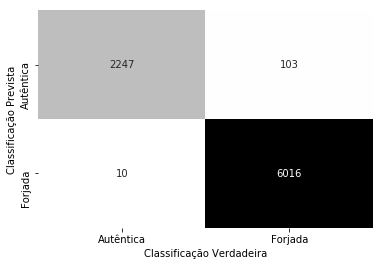
\includegraphics[width=\linewidth]{img/matriz-lenet-a}
      \end{subfigure}
      \hspace{2cm}
      \begin{subfigure}{0.25\linewidth}
        \caption{LeNet B}
        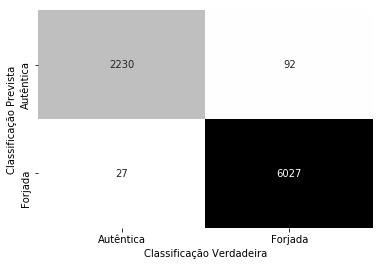
\includegraphics[width=\linewidth]{img/matriz-lenet-b}%
      \end{subfigure}

      \begin{subfigure}{0.25\linewidth}
        \caption{LeNet C}
        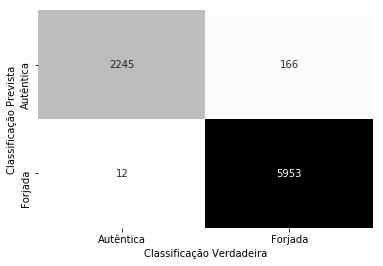
\includegraphics[width=\linewidth]{img/matriz-lenet-c}%
      \end{subfigure}
      \hspace{2cm}
      \begin{subfigure}{0.25\linewidth}
        \caption{LeNet D}
        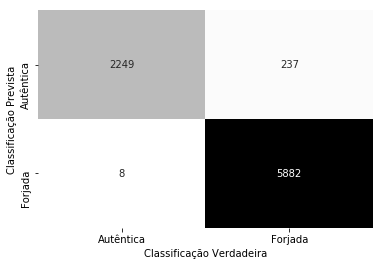
\includegraphics[width=\linewidth]{img/matriz-lenet-d}%
      \end{subfigure}
  \end{figure}
\end{frame}


\begin{frame}{AlexNet}

  \begin{table}[h!]
\centering
\caption{Detalhamento dos melhores modelos obtidos com a arquitetura AlexNet.}
\label{tab:alexnet}
\begin{tabular}{cccccc}
\toprule
\textbf{Identificação} & \textbf{Otimizador} & \textbf{\emph{Patience}}  & \textbf{Função de Ativação} & \textbf{Acurácia} & \textbf{F-Score} \\
\midrule
AlexNet A & Adam & 15 & ELU & $0.9654$ & $0.9393$ \\
AlexNet B & SGD & 10 & \emph{Leaky} ReLU & $0.9601$ & $0.9311$ \\
AlexNet C & SGD & 5 & SELU & $0.9561$ & $0.9244$ \\
\bottomrule
\end{tabular}
\end{table}

\end{frame}

\begin{frame}{AlexNet}

  \begin{figure}[ht!]
      \caption{Histórico de \emph{loss} e acurácia durante o treinamento dos melhores modelos obtidos com a arquitetura AlexNet.}\label{fig:alexnet-treinamento}
      \begin{subfigure}[hb]{0.4\linewidth}
        \caption{\emph{Loss} durante o treinamento da AlexNet A}
        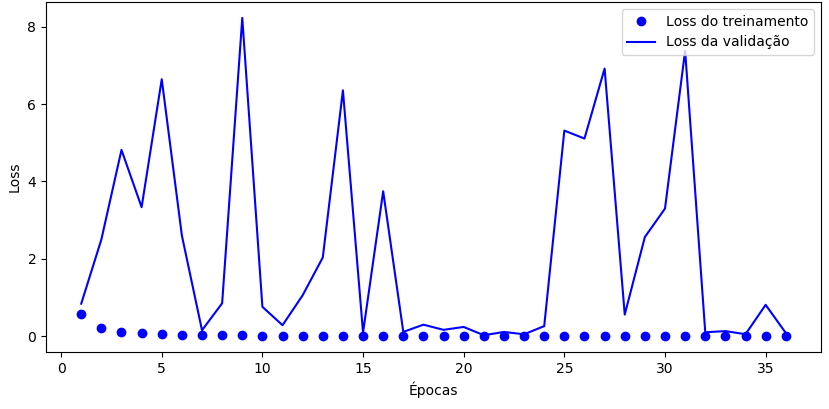
\includegraphics[width=\linewidth]{img/alexnet-a-loss}
      \end{subfigure}
      \hspace{2cm}
      \begin{subfigure}[hb]{0.4\linewidth}
        \caption{Acurácia durante o treinamento da AlexNet A}
        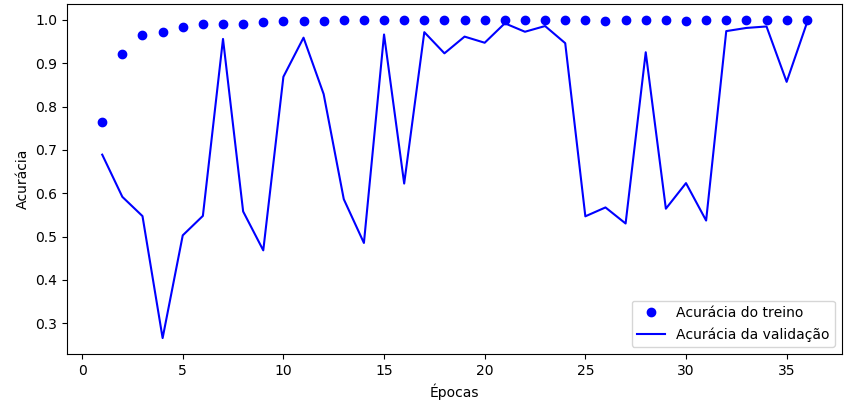
\includegraphics[width=\linewidth]{img/alexnet-a-acc}%
      \end{subfigure}
  \end{figure}
\end{frame}

\begin{frame}{AlexNet}
  \vskip1\baselineskip
  \begin{figure}[ht!]
      \caption{Matrizes de confusão dos melhores modelos obtidos com a arquitetura AlexNet.}\label{fig:matrizes-alexnet}
      \begin{subfigure}[hb]{0.3\linewidth}
        \caption{AlexNet A}
        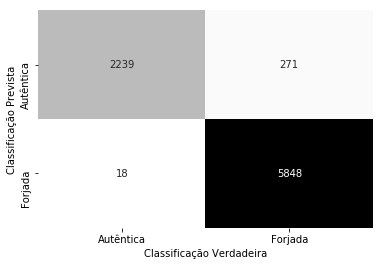
\includegraphics[width=\linewidth]{img/matriz-alexnet-a}
      \end{subfigure}
      \hspace{0.5cm}
      \begin{subfigure}{0.3\linewidth}
        \caption{AlexNet B}
        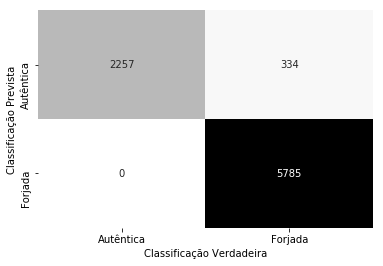
\includegraphics[width=\linewidth]{img/matriz-alexnet-b}%
      \end{subfigure}
      \hspace{0.5cm}
      \begin{subfigure}{0.3\linewidth}
        \caption{AlexNet C}
        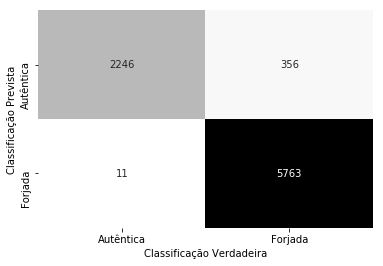
\includegraphics[width=\linewidth]{img/matriz-alexnet-c}%
      \end{subfigure}
  \end{figure}
\end{frame}
